\documentclass[14pt,a4paper]{article}

\usepackage[russian]{babel} % Русский язык
\usepackage{geometry} % Установка полей
\usepackage{graphicx} % Пакет для работы с изображениями
\usepackage{verbatim} % для вставки текста без интерпретации его как LaTeX-команд
\usepackage[hidelinks]{hyperref}

\geometry{top=2cm, bottom=2cm, left=3cm, right=1.5cm}

\begin{document}
% Титульный лист
\begin{titlepage}
  \begin{center}
    {\large\scshape\bfseries
    МИНИСТЕРСТВО НАУКИ И ВЫСШЕГО ОБРАЗОВАНИЯ РОССИЙСКОЙ ФЕДЕРАЦИИ\\
    ФЕДЕРАЛЬНОЕ ГОСУДАРСТВЕННОЕ АВТОНОМНОЕ ОБРАЗОВАТЕЛЬНОЕ УЧРЕЖДЕНИЕ ВЫСШЕГО ОБРАЗОВАНИЯ\\
    «СЕВЕРО-КАВКАЗСКИЙ ФЕДЕРАЛЬНЫЙ УНИВЕРСИТЕТ»\\
    ФАКУЛЬТЕТ МАТЕМАТИКИ И КОМПЬЮТЕРНЫХ НАУК ИМЕНИ ПРОФЕССОРА Н.И.ЧЕРВЯКОВА}
    \vfill
    \Large{\textbf{ЛАБОРАТОРНАЯ РАБОТА №15}}\\[2mm]
    \large{Алгоритмизация и программирование}\\[6mm]
    \large{\textbf{Файлы}}\\[20mm]
  \end{center}
  \begin{flushright}
    \textbf{Выполнил студент:}\\
    Сивко Иван Андреевич\\
    студент 2 курса\\
    группа ПМИ-б-о-23-2,\\
    направление подготовки 01.03.02\\[5mm]
    \textbf{Проверил:}\\
    Ассистент кафедры вычислительной\\
    математики и кибернетики, к.ф.-м.н.,\\
    Черкашина Анастасия Андреевна
  \end{flushright}
  \vfill
  \begin{center}
    \the\year\ г.
  \end{center}
\end{titlepage}

% \tableofcontents
% \newpage

% Основная часть
\begin{center}
  \textbf{Вариант 9}
\end{center}
{\large {\bfseries Цель:} Совершенствование навыков в программировании с использованием\\ указателей.}

\pdfbookmark[1]{Задание 1}{sec1}
\section*{Задание 1}
\textbf{Работа с неструктурированными данными}
\renewcommand{\thesubsection}{\arabic{subsection}} % Задания нумерации для \subsection
\setcounter{subsection}{0} % подпункты с 1
\subsection{Условие}
Для исследования различных методов доступа к файлам данных необходимо выполнить следующие подготовительные действия:

\begin{enumerate}
  \item \textbf{Создайте текстовый файл.}

    Содержимое файла:
    \begin{quote}
      У меня спросили: сколько будет x Опер y?\\
      А я не знаю! А n Опер k? Тоже!\\
      Помогите!
    \end{quote}
    Например:
    \begin{quote}
      У меня спросили: сколько будет 7 * 2?\\
      А я не знаю! А 9 / 4? Тоже!\\
      Помогите!
    \end{quote}
    Создайте файл с указанным содержимым в текстовом редакторе (например, в Блокноте).

  \item \textbf{Обработайте данные.}

    Вам известна структура файла. Необходимо:
    \begin{itemize}
      \item Вывести содержимое файла на экран.
      \item Записать в выходной файл результаты в формате:
    \end{itemize}
    \begin{quote}
      x Опер y = Рез1\\
      n Опер k = Рез2
    \end{quote}
    Например:
    \begin{quote}
      7 * 2 = 14\\
      9 / 4 = 2.25
    \end{quote}
  \item Исходные данные берутся из таблицы согласно варианта:
    \begin{figure}[h]
      \centering
      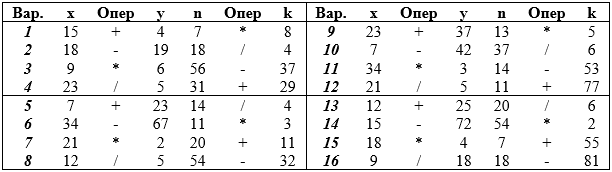
\includegraphics[width=0.8\textwidth]{data/condition15_1.png} % Укажите имя файла изображения
    \end{figure}
\end{enumerate}

\subsection{Код:}

\verbatiminput{data/task15_1.c}
\subsection{Результат работы программы}
\begin{figure}[h]
  \centering
  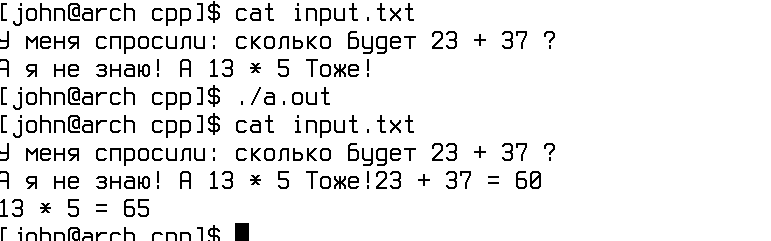
\includegraphics[width=0.8\textwidth]{data/demo15_1.png} % Укажите имя файла изображения
\end{figure}

\pdfbookmark[1]{Задание 2}{sec2}
\section*{Задание 2}
\textbf{Работа со структурированными данными}
\setcounter{subsection}{0}
\subsection{Условие}
Используя полученную при выполнении лабораторной работы 14 программу, реализовать возможность сохранения данных в файл с последующим чтением из файла введенных данных.
\subsection{Код:}
\verbatiminput{data/task15_2.c}
\subsection{Результат работы программы:}
\begin{figure}[h]
  \centering
  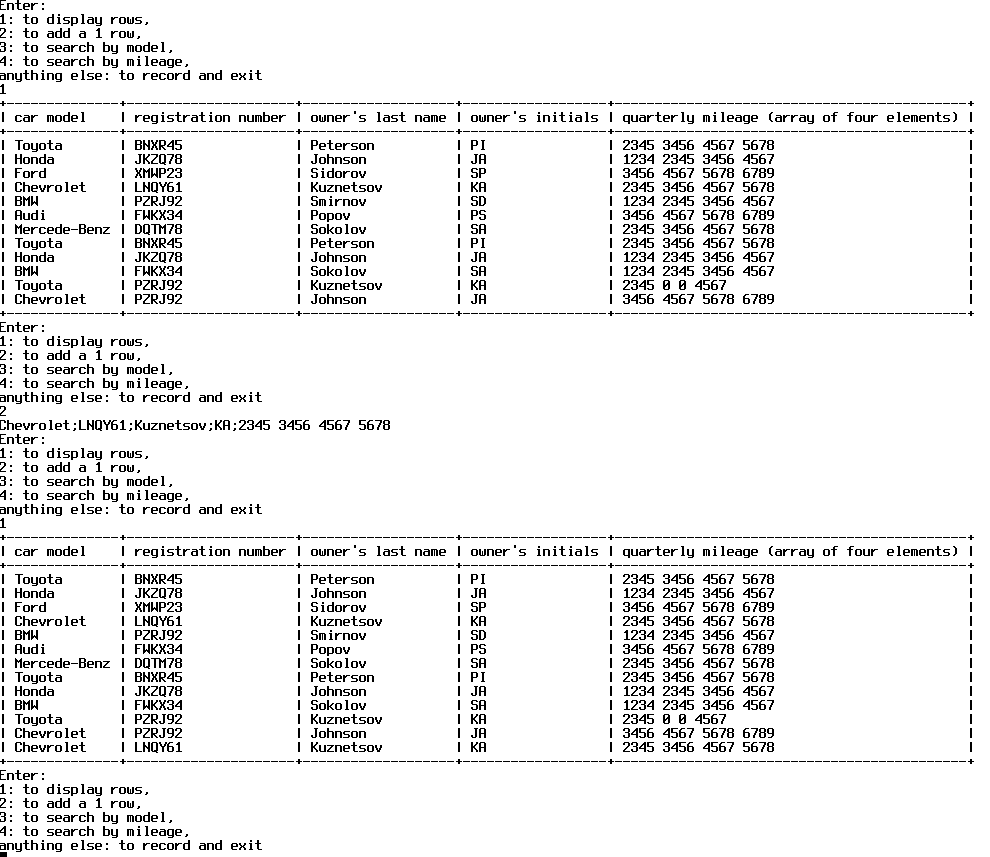
\includegraphics[width=0.8\textwidth]{data/demo15_2.png} % Укажите имя файла изображения
\end{figure}
\begin{figure}[h]
  \centering
  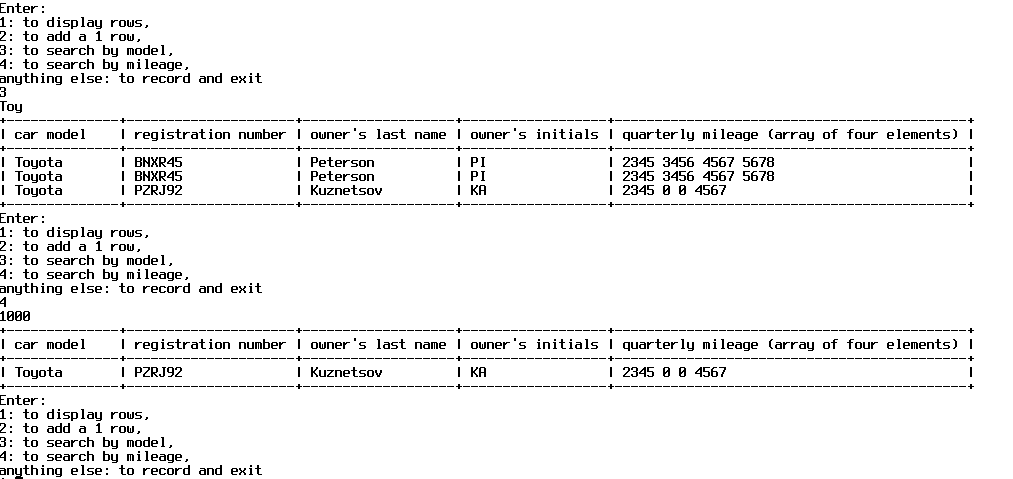
\includegraphics[width=0.8\textwidth]{data/demo15_2_2.png} % Укажите имя файла изображения
\end{figure}
\newpage

\section*{Задание 3}
\setcounter{subsection}{0}
\subsection{Условие}
В соответствии с вариантом написать и отладить программу:

Дана информация о пяти больных. Структура имеет вид: фамилия, возраст, пол, давление. Вывести данные о больных с повышенным давлением (более 140) и подсчитать их количество.
\subsection{Код:}
\verbatiminput{data/task15_3.c}
\newpage
\subsection{Результат работы программы:}
\begin{figure}[h]
  \centering
  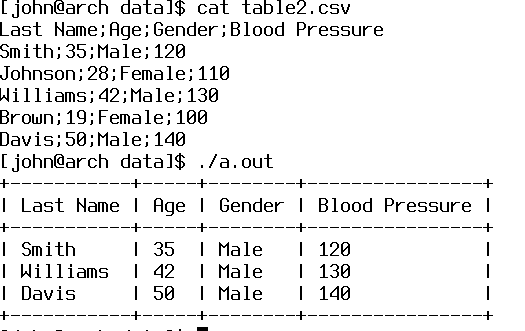
\includegraphics[width=0.8\textwidth]{data/demo15_3.png} % Укажите имя файла изображения
\end{figure}
\end{document}
